\documentclass{subfiles}

\begin{document}
\section{Time-evolution of quantum gate protocols}\label{sec:time_evolution}
We simulate the time-dependent Schrödinger equation for two distinguishable particles in our double-well Morse potential, in accordance with the procedural framework outlined in Section \ref{sec:summary_workflow}. The system is built in the Sinc-DVR basis using, and mapped into the reduced Hartree basis as described in Section \ref{sec:Hartree_method}. We choose eigenvectors of Hamiltonian in the optimal parameters for configuation $C_I$ as our measurement (computational) basis, as the eigenvectors of this configuration have complete overlap with the logical basis states $\ket{ij}$, i.e the product states of the two particles. Our ramping protocol (Section \ref{sec:ramping_protocol}) smoothly ramps from configuration $C_I$ (non-degenerate qubit levels, zero entanglement) to configuration $C_{II}$ (close-to degeneracy in first excitations, high entanglement), and back. In what follows, we present the results of our time-evolution simulations, focusing on the state populations throughout. First we shall present a minimal "two-level" model of the system ($l=2$ basis functions per well) to demonstrate the idealized gate action and entanglement generation, and then we will present the full simulation ($l=4$ basis functions per well) to investigate the effects of higher-order excitations, assess higher-order leakage and its impact on gate fidelity. The discussions that follow will focus on the implications of these results for quantum control protocols and the feasibility of implementing a two-qubit gate operation in a real-world experimental setup. Time-scales in the simulations are given in atomic units (a.u.), where $1$ a.u. corresponds to approximately $2.42 \times 10^{-17}$ seconds (Hartree time), or about $58.7$ attoseconds. The total simulation times will be converted as needed to SI units, and the time steps are set to $\Delta t = 0.1$ a.u. for all simulations, ensuring a sufficiently fine resolution for capturing the dynamics of the system.

\subsection{Two-level model: Idealized gate action and entanglement generation}
In the reduced four-dimensional Hilbert space spanned by the product states $\{\ket{00}, \ket{01}, \ket{10}, \ket{11}\}$, we simulate the time evolution using the unitary time-evolution operator (Section \ref{sec:time_evolution_operator}) for the two-particle system. Because only the first four states are active, there is no possibility for population leakage to higher order states outside the qubit subspace, and we can expect the system to behave as a perfect two-qubit gate. Figure \ref{fig:time_evolution_2_basefunctions} shows the time evolution of the state populations for the two-level model, where we've plotted the populations 
\begin{align*}
    P_{ij} = |\braket{ij| \psi(t)}|^2,
\end{align*}
for each logical state $\ket{ij}$ in the qubit manifold, as a function of time.
\begin{figure}[h!]
    \centering
    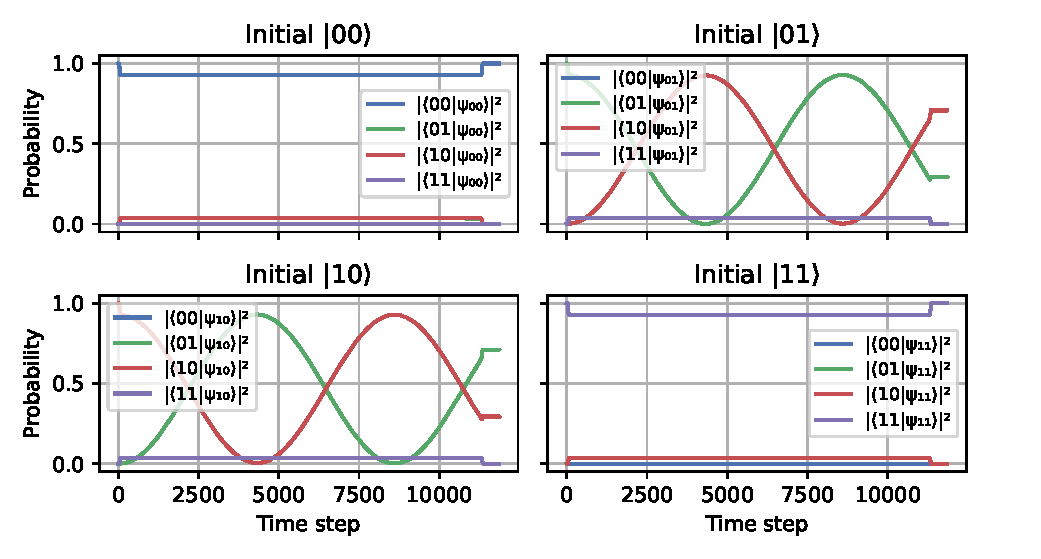
\includegraphics[width=1.0\textwidth]{figs/time_evolution_2_basefunctions_1806.pdf}
    \caption{Evolution of the state populations for the two-level model of the Morse double-well potential, showing the idealized gate action and entanglement generation. The populations of the logical states $\ket{10}$ and $\ket{01}$ oscillate in a coherent manner, indicating a successful SWAP-like operation. The populations of the states $\ket{00}$ and $\ket{11}$ remain constant. The parameters used for the ramping protocol are $T_{\text{start}} = 10.0$ a.u., $T_{\text{end}} = 500.0$ a.u, $T_{\text{up}} = 50.0$ a.u., $T_{\text{down}} = 50.0$ a.u., and the hold time $T_{\text{hold}} = 11125.0$ a.u. The ramping protocol is applied to the Morse double-well potential parameters for configuration $C_I$ and $C_{II}$, as described in Section \ref{sec:optimization_result}. The simulation is run for a total time of $T_{\text{total}} = 11860.0$ a.u., with a time step of $\Delta t = 0.1$ a.u. Converted using the atomic units, this corresponds to a total time $T_{\text{total}}=0.287$ picoseconds. \textcolor{red}{TODO: Maybe re-do figure to get better swap? Or should we save that to the full system perhaps?}}
    \label{fig:time_evolution_2_basefunctions}
\end{figure}
\\ 

The figure shows how the populations initially is clearly separated, with clean energy eigenfunctions (e.g $\braket{\psi_0(0)|00} = 1$), before the ramping procedure is initiated at $t = 50.0$ a.u. During the ramp we see a slight nudge in the populations, where there is some leakage between states but this is negligable. After ramp is completeted, the 1st and 2nd excited states $\psi_1(t)$ and $\psi_2(t)$, initially in $\ket{01}$ and $\ket{10}$ respectively, oscillate coherently between the two states, indicating a successful SWAP-like operation. The entanglement is generated as the populations of the two energy eigenstates mix, and swap, with a uniform frequency of oscillation. This clean SWAP-like behaviour serves as a proof of concept for the two-qubit gate operation in our Morse double-well potential, demonstrating that the system can be controlled to perform a coherent mixing of the logical states $\ket{10}$ and $\ket{01}$, thus generating entanglement. At the end of the simulation the energy eigenfunctions are in a superposition,
\begin{align*}
    \ket{\psi_1(t_{\text{end}})} &\approx 0.2885 \ket{01} + 0.7115 \ket{10}, \\
    \ket{\psi_2(t_{\text{end}})} &\approx 0.7115 \ket{01} + 0.2885 \ket{10},
\end{align*}
with negligible contributions from the states $\ket{00}$ and $\ket{11}$, which remain (almost) constant throughout the simulation. To improve upon this result, we can investigate various time-scales for the simulation.

We also identify the importance of optimizing the ramping procedure to ensure that the populations of the states $\ket{00}$ and $\ket{11}$ remain consistent with our desired gate operation post ramp, as the populations oscillates in time. Carefully constructed ramping protocols can be the difference between a succesful (total) swap between the two states, a perfect mixing where the two states are equally populated, or a failed operation where the states go back to their original population after the gate operation has been performed. Due to the simple nature of the two-level model, we used the direct matrix exponentiation method to compute the time-evolution operator, which is efficient and fast for smaller systems. 
\textcolor{red}{TODO: Add more discussions? We should also check the fidelity of the gate, i.e, what is the Unitary matrix at the end of our simulation - does it correspond to a perfect SWAP gate? We must also quantify the population of states at $t_{\text{end}}$ and add that to our discussion to show the success beyond just the qualitative analysis of the plot.}


\subsection{Four-level model: Higher-order excitations and gate fidelity}
In the four-level model, we include higher-order excitations by using $l=4$ basis functions per well, allowing us to investigate the effects of higher-order excitations on the gate operation, and reveal realistic limitations of the two-qubit gate operation in our Morse double-well potential. We must now optimize more carefully to avoid off-diagonal couplings that lead to leakage to higher-order states that would otherwise spoil the two-qubit gate protocol. Leakage between the qubit manifold $\{\ket{01}, \ket{10}\}$ and the higher-order spectator manifolds can lead to unwanted population transfer, instability during evolution, and de-phasing effects that can significantly reduce the fidelity of the gate
operation. \textcolor{red}{TODO: ADd more on this discuttion, and maybe move to the end of section?: "There is also the aspect of optimizing the ramping protocol to avoid non-ideal transitions and de-phasing, and the trade-off between between adiabaticity and speed will be the subject of further studies." }
\subsubsection*{SWAP-gate operation}
\begin{figure}[h!]
    \centering
    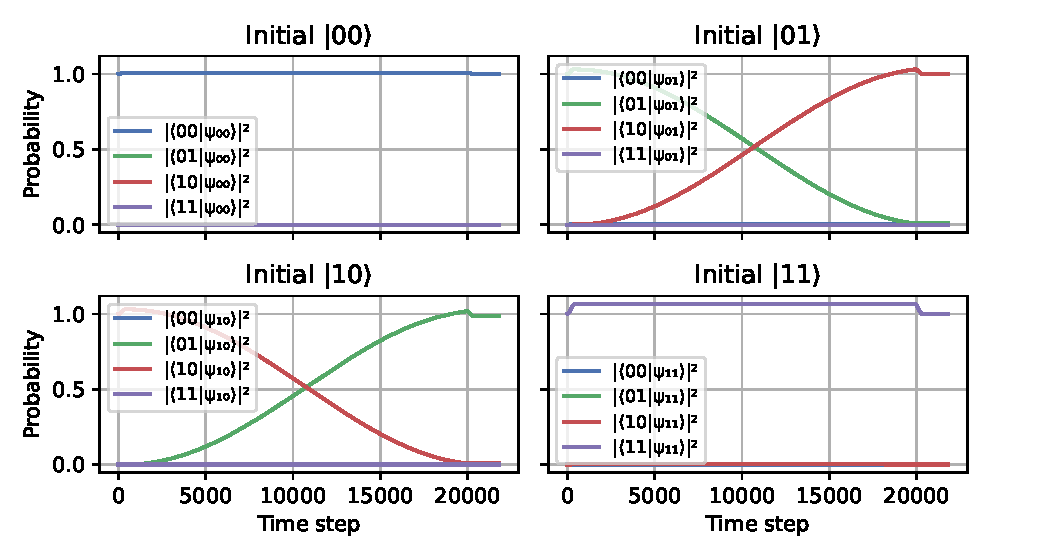
\includegraphics[width=1.0\textwidth]{figs/time_evolution_4_basefunctions_2206_2nd.pdf}
    \caption{Evolution of the state populations for the four-level model of the Morse double-well potential using the CN integrator, showing the effects of higher-order excitations on the gate operation. The populations of the energy eigenstates $\ket{\psi_0(t)}$ and $\ket{\psi_1(t)}$ oscillate in a coherent manner, but due to the low coupling term $J=H[\psi_0, \psi_1]$ the oscillations are elongated. The coherent oscillations do indicate successful SWAP-like operation, but we note that the mixture is not clean. During evolution, there is possibly some leakage to higher order states not present in the plot.
    The parameters used in the ramping protocol are $T_{\text{start}} = 10.0$ a.u., $T_{\text{end}} = 1500.0$ a.u, $T_{\text{up}} = 500.0$ a.u., $T_{\text{down}} = 500.0$ a.u., and the hold time $T_{\text{hold}} = 19 315.0$ a.u. The ramping protocol is applied to the Morse double-well potential parameters for configuration $C_I$ and $C_{II}$, as described in Section \ref{sec:optimization_result}. The simulation is run for a total time of $T_{\text{total}} \approx 22 000.0$ a.u., with a time step of $\Delta t = 0.1$ a.u. Converted using the atomic units, this corresponds to a total time $T_{\text{total}}=0.53$ picoseconds. \textcolor{red}{TODO: Re-do this calculation in effective SI-units? More time, approx 1 a.u. $=60$ femtoseconds from the effective bohr radii used in distinguishable study}
    }
    \label{fig:time_evolution_4_basefunctions}
\end{figure}
In figure \ref{fig:time_evolution_4_basefunctions} we show the time evolution of the state populations for the four-level model, where we observe similar behaviour as in the idealised two-level model, but with some leakage to higher-order states. The populations of the eigenstates $\ket{\psi_0(t)}$ and $\ket{\psi_1(t)}$ oscillate in a coherent manner, indicating a successful SWAP-like operation. The final state population of the two energy eigenstates are
\begin{align*}
    \ket{\psi_1(t_{\text{end}})} &\approx 0.9863 \ket{01} + 0.0072 \ket{10}  \\
    \ket{\psi_2(t_{\text{end}})} &\approx 0.0072 \ket{01} + 0.9993 \ket{10},
\end{align*}
and we note that there is some minor leakage to higher order states - which is why they are approximations. 
\\
Figure \ref{fig:time_evolution_4_basefunctions} shows the protocol with hold time to approximately match the Rabi oscillation for a successful swap of the logical states. I.e since the Rabi oscillation frequency is given by the coupling term $J = H[\psi_1, \psi_2]$, through $P_{01\to10} = \sin^2(J t)$, we can optimize the hold time to be a multiple of the Rabi oscillation period $T_R = \pi/(4J)$. With a coupling term of $J = 7.9674 \times 10^{-5}$ a.u., we find the Rabi oscillation period to be $T_R 19715 $ a.u., and we set the hold time accordingly. We note that the oscillations are elongated compared to the two-level model, indicating that the coupling term is lower than in the idealized case. This is expected, as we have higher-order excitations that can lead to leakage and de-phasing effects. \textcolor{red}{TODO: Add more discussion and move onto physical realisation of this evolution}


To assess how this evolution aligns with our desired SWAP gate operation, we can compute the logical propagator $U_{\text{logical}}$\textcolor{red}{TODO: Should add a small note in theory/method section for this?},
\begin{align*}
    U_{\text{logical}} = \Psi_0^\dagger\Psi(t_f) = \begin{pmatrix}
        \braket{00|\psi_00(t_f)} & \braket{00|\psi_01(t_f)} & \braket{00|\psi_10(t_f)} & \braket{00|\psi_11(t_f)} \\
        \braket{01|\psi_00(t_f)} & \braket{01|\psi_01(t_f)} & \braket{01|\psi_10(t_f)} & \braket{01|\psi_11(t_f)} \\
        \braket{10|\psi_00(t_f)} & \braket{10|\psi_01(t_f)} & \braket{10|\psi_10(t_f)} & \braket{10|\psi_11(t_f)} \\
        \braket{11|\psi_00(t_f)} & \braket{11|\psi_01(t_f)} & \braket{11|\psi_10(t_f)} & \braket{11|\psi_11(t_f)}
    \end{pmatrix},
\end{align*}
where $\Psi(t_f)$ is the time-evolved wavefunction at the end of the simulation, and $\Psi_0$ is the initial wavefunction in the logical basis. The ideal SWAP gate operation would yield a propagator of the form \eqref{eq:swap_gate}, i.e
\begin{align*}
    U_{\text{ideal}} = \begin{pmatrix}
        1 & 0 & 0 & 0 \\
        0 & 0 & 1 & 0 \\
        0 & 1 & 0 & 0 \\
        0 & 0 & 0 & 1
    \end{pmatrix}.
\end{align*}
The result of our simulation yields the following logical propagator,
\begin{align*}
U_{\text{logical}}
&=
\begin{pmatrix}
-0.8490 + 0.5284i &  0.0000 + 0.0000i &  0.0000 - 0.0000i &  0.0000 + 0.0000i \\
-0.0000 - 0.0000i &  0.0613 - 0.0593i &  0.0028 - 0.9931i & -0.0000 - 0.0000i \\
 0.0000 - 0.0000i & -0.6230 + 0.7817i & -0.0107 - 0.0846i &  0.0000 - 0.0000i \\
 0.0000 + 0.0000i & -0.0000 + 0.0000i &  0.0000 + 0.0000i & -0.9768 - 0.2140i
\end{pmatrix},\\[1ex]
\lvert U_{\text{logical}}\rvert^2
&=
\begin{pmatrix}
1.0000 & 0.0000 & 0.0000 & 0.0000 \\
0.0000 & 0.0073 & 0.9863 & 0.0000 \\
0.0000 & 0.9992 & 0.0073 & 0.0000 \\
0.0000 & 0.0000 & 0.0000 & 0.9999
\end{pmatrix}.
\end{align*}
We can see that the propagator is close to the ideal SWAP gate operation, with the populations of the states $\ket{00}$ and $\ket{11}$ remaining constant, while swapping the populations of the states $\ket{\psi_1}$  (initially $\ket{01}$) and $\ket{\psi_2}$ (initially $\ket{10}$) almost perfectly, to an accuracy of $99.92\%$ and $98.63\%$ respectively. The small deviations can be improved upon by further optimizing the ramping protocol. We can further assess the fidelity by computing the average and classical fidelity of the gate operation \textcolor{red}{TODO: Should add this also, an equation, in theory/method}, recalling its definition as
\begin{align*}
    F = \frac{|\text{Tr}(U_{\text{ideal}}^\dagger U_{\text{logical}})|^2 + d}{d(d+1)},
\end{align*}
where $d$ is the dimension of the logical sub-space, which in our case is $d=4$. The average fidelity of our gate operation is computed to be $F = 49.97\%$. This indicates that while the gate operation is not perfect, it is still a significant improvement over random operations, which would yield an average fidelity of $F = 25\%$. The deviation from the ideal SWAP gate operation arises from the fact that we do not optimize with regards to the phase evolution of the states, and instead only focus on the population transfer between the states. A better measurement of the gate performance as we have optimized for, would be the classical fidelity\textcolor{red}{TODO: Add this to theory/method section?}, defined as
\begin{align*}
    F_c = \frac{1}{d} \sum_{i=0}^{d-1} |\braket{\psi_i | \psi_i(t_f)}|^2.
\end{align*}
Computed for our simulation, we find the classical fidelity to be $F_c = 99.64\%$, indicating that the gate operation is indeed successful in transferring the populations of the states $\ket{01}$ and $\ket{10}$, even without much optimization of the ramping protocol, and only an approximation of the Rabi oscillation is used. 

\subsubsection*{$\sqrt{\text{SWAP}}$-gate operation}
In addition to the SWAP gate operation, we can also investigate the $\sqrt{\text{SWAP}}$ gate operation, which is a half-SWAP operation that transfers only half of the population from one state to another, inducing maximally entangled Bell-states\eqref{eq:bell_states} at the end of the operation. 
\begin{figure}[h!]
    \centering
    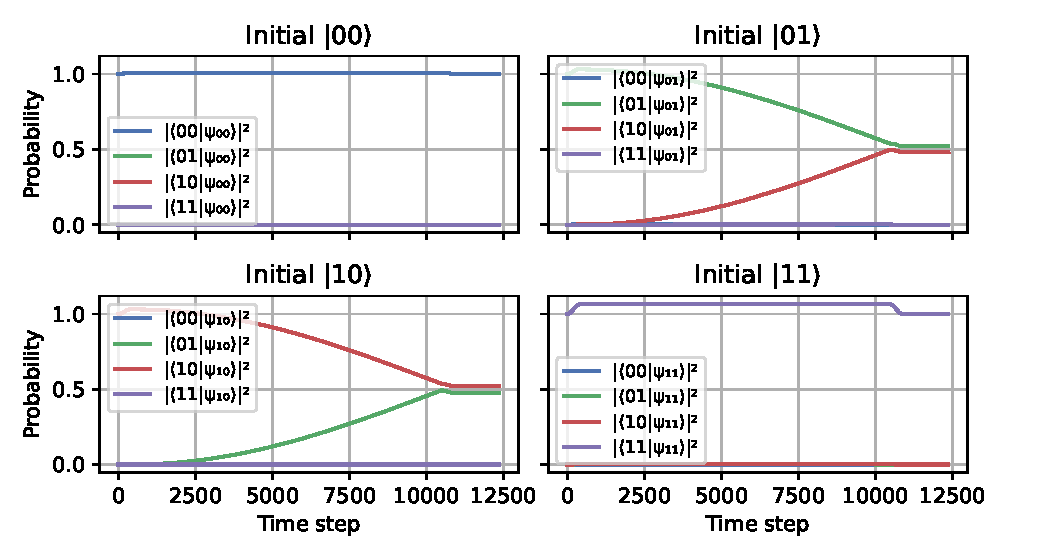
\includegraphics[width=1.0\textwidth]{figs/time_evolution_4_basefunctions_2206_squareSWAP.pdf}
    \caption{Evolution of the state populations in the four-level model of the Morse double-well potential using the CN integrator, showing the $\sqrt{\text{SWAP}}$ gate operation. The evolution is with a hold time $T_{\text{hold}} = T_{\text{SWAP}}/2 = 9857$ a.u. The ramp up and down times are set to $T_{\text{up}} = T_{\text{down}} = 500$ a.u., and we end with $T_{\text{end}} = 1500$ a.u. We see that running the evolution for a half-Swap duration results in a near-perfect mixed state, and we get Bell-like states for the first two energy eigenstates, while the remaining states remain constant. Qualitatively, this looks like we have implemented a successful $\sqrt{\text{SWAP}}$ gate-like operation, where the populations of the states $\ket{01}$ and $\ket{10}$ are mixed.}
    \label{fig:time_evolution_4_basefunctions_sqrtSWAP}
\end{figure}
Figure \ref{fig:time_evolution_4_basefunctions_sqrtSWAP} shows the time-evolution of the same system as in figure \ref{fig:time_evolution_4_basefunctions}, but with a hold time of $T_{\text{hold}} = T_{\text{SWAP}}/2 = 9857$ a.u., which is half the Rabi oscillation period. To this end, we aim to achieve a $\sqrt{\text{SWAP}}$ gate operation, which would yield a maximally entangled Bell-state at the end of the operation. Qualitatively, we see that the population of the states $\ket{01}$ and $\ket{10}$ are highly mixed, indicating that we've been successful to some degree. At the end of simulation, the populations of the two energy eigenstates are
\begin{align*}
    \ket{\psi_1(t_{\text{end}})} &\approx 0.4765 \ket{01} + 0.5203 \ket{10}, \\
    \ket{\psi_2(t_{\text{end}})} &\approx 0.5203 \ket{01} + 0.4828 \ket{10},
\end{align*}
which means we have achieved a good mixing of the two states, but not a perfect $\sqrt{\text{SWAP}}$ gate, altough the states $\psi_0(t)$ and $\psi_3(t)$ remain constant (to an accuracy of $10^{-5}$). We can note that we've succesfully implemented a $\sqrt{\text{SWAP}}$ gate-like operation, where the populations of the states $\ket{01}$ and $\ket{10}$ are mixed, but not to the extent that we achieve a perfect Bell-state. 
To quantitatively assess the success of the $\sqrt{\text{SWAP}}$ gate operation, we can compute the logical propagator $U_{\text{logical}}$ as before, and compare it to the ideal $\sqrt{\text{SWAP}}$ gate operation. Recall, the ideal $\sqrt{\text{SWAP}}$ \ref{eq:sqrt_swap_gate} is given by 
\begin{align*}
    U_{\sqrt{\text{SWAP}}} = \frac{1}{{2}}\begin{pmatrix}
        1 & 0 & 0 & 0 \\
        0 & 1 + i & 1 - i & 0 \\
        0 & 1 - i & 1 + i & 0 \\
        0 & 0 & 0 & 1
    \end{pmatrix}.
\end{align*}
The result of our simulation yields
\begin{equation}
U_{\mathrm{logical}}
=\begin{pmatrix}
 0.9635 + 0.2677i & -0.0000 + 0.0000i & -0.0000 - 0.0000i &  0.0000 - 0.0000i\\
 0.0000 - 0.0000i &  0.1459 - 0.7066i & -0.4457 - 0.5269i & -0.0000 + 0.0000i\\
-0.0000 - 0.0000i &  0.0217 + 0.6943i & -0.5814 - 0.4273i &  0.0000 - 0.0000i\\
 0.0000 - 0.0000i & -0.0000 + 0.0000i &  0.0000 - 0.0000i & -0.8709 + 0.4914i
\end{pmatrix}.
\end{equation}
Of which, if we take the element-wise modulus, we gain the population transfer matrix
\begin{equation}
\sqrt{\lvert U_{\mathrm{logical}}\rvert^2}
=\begin{pmatrix}
1.0000 & 0.0000 & 0.0000 & 0.0000\\
0.0000 & 0.7215 & 0.6901 & 0.0000\\
0.0000 & 0.6947 & 0.7215 & 0.0000\\
0.0000 & 0.0000 & 0.0000 & 1.0000
\end{pmatrix}.
\end{equation}
Calculating the gate fidelity, we find the classical fidelity to be $F_c = 73.97\%$, indicating that the gate works but is not perfect. As before, the lack of phase control throughout evolution hurts the gate fidelity, and we can improve upon this by optimizing the ramping protocol to ensure that the relative phases of the states are preserved throughout the evolution. As we are more interested in the realisation of correct population transfer, we can instead assess the fidelity of the population transfer matrix, which is given by $|U_{\sqrt{\text{SWAP}}}|$, which yields a classical fidelity of $F_c = 75.51\%$. \textcolor{red}{TODO: We omit the average fidelity here, as it is $\approx 25\%$ - which is not particularly impressive. Should we add it anyway for consistency?}











\end{document}